\documentclass[11pt, a5paper, parskip=half-, DIV=12]{scrartcl}

\usepackage{../endeavour}
\usepackage{../endeavour_book}

\version{0.1}

\begin{document}
% Colour Cover
\thispagestyle{plain}
\AddToShipoutPictureBG{
\begin{tikzpicture}[remember picture, overlay]
	\node () at (current page.center) {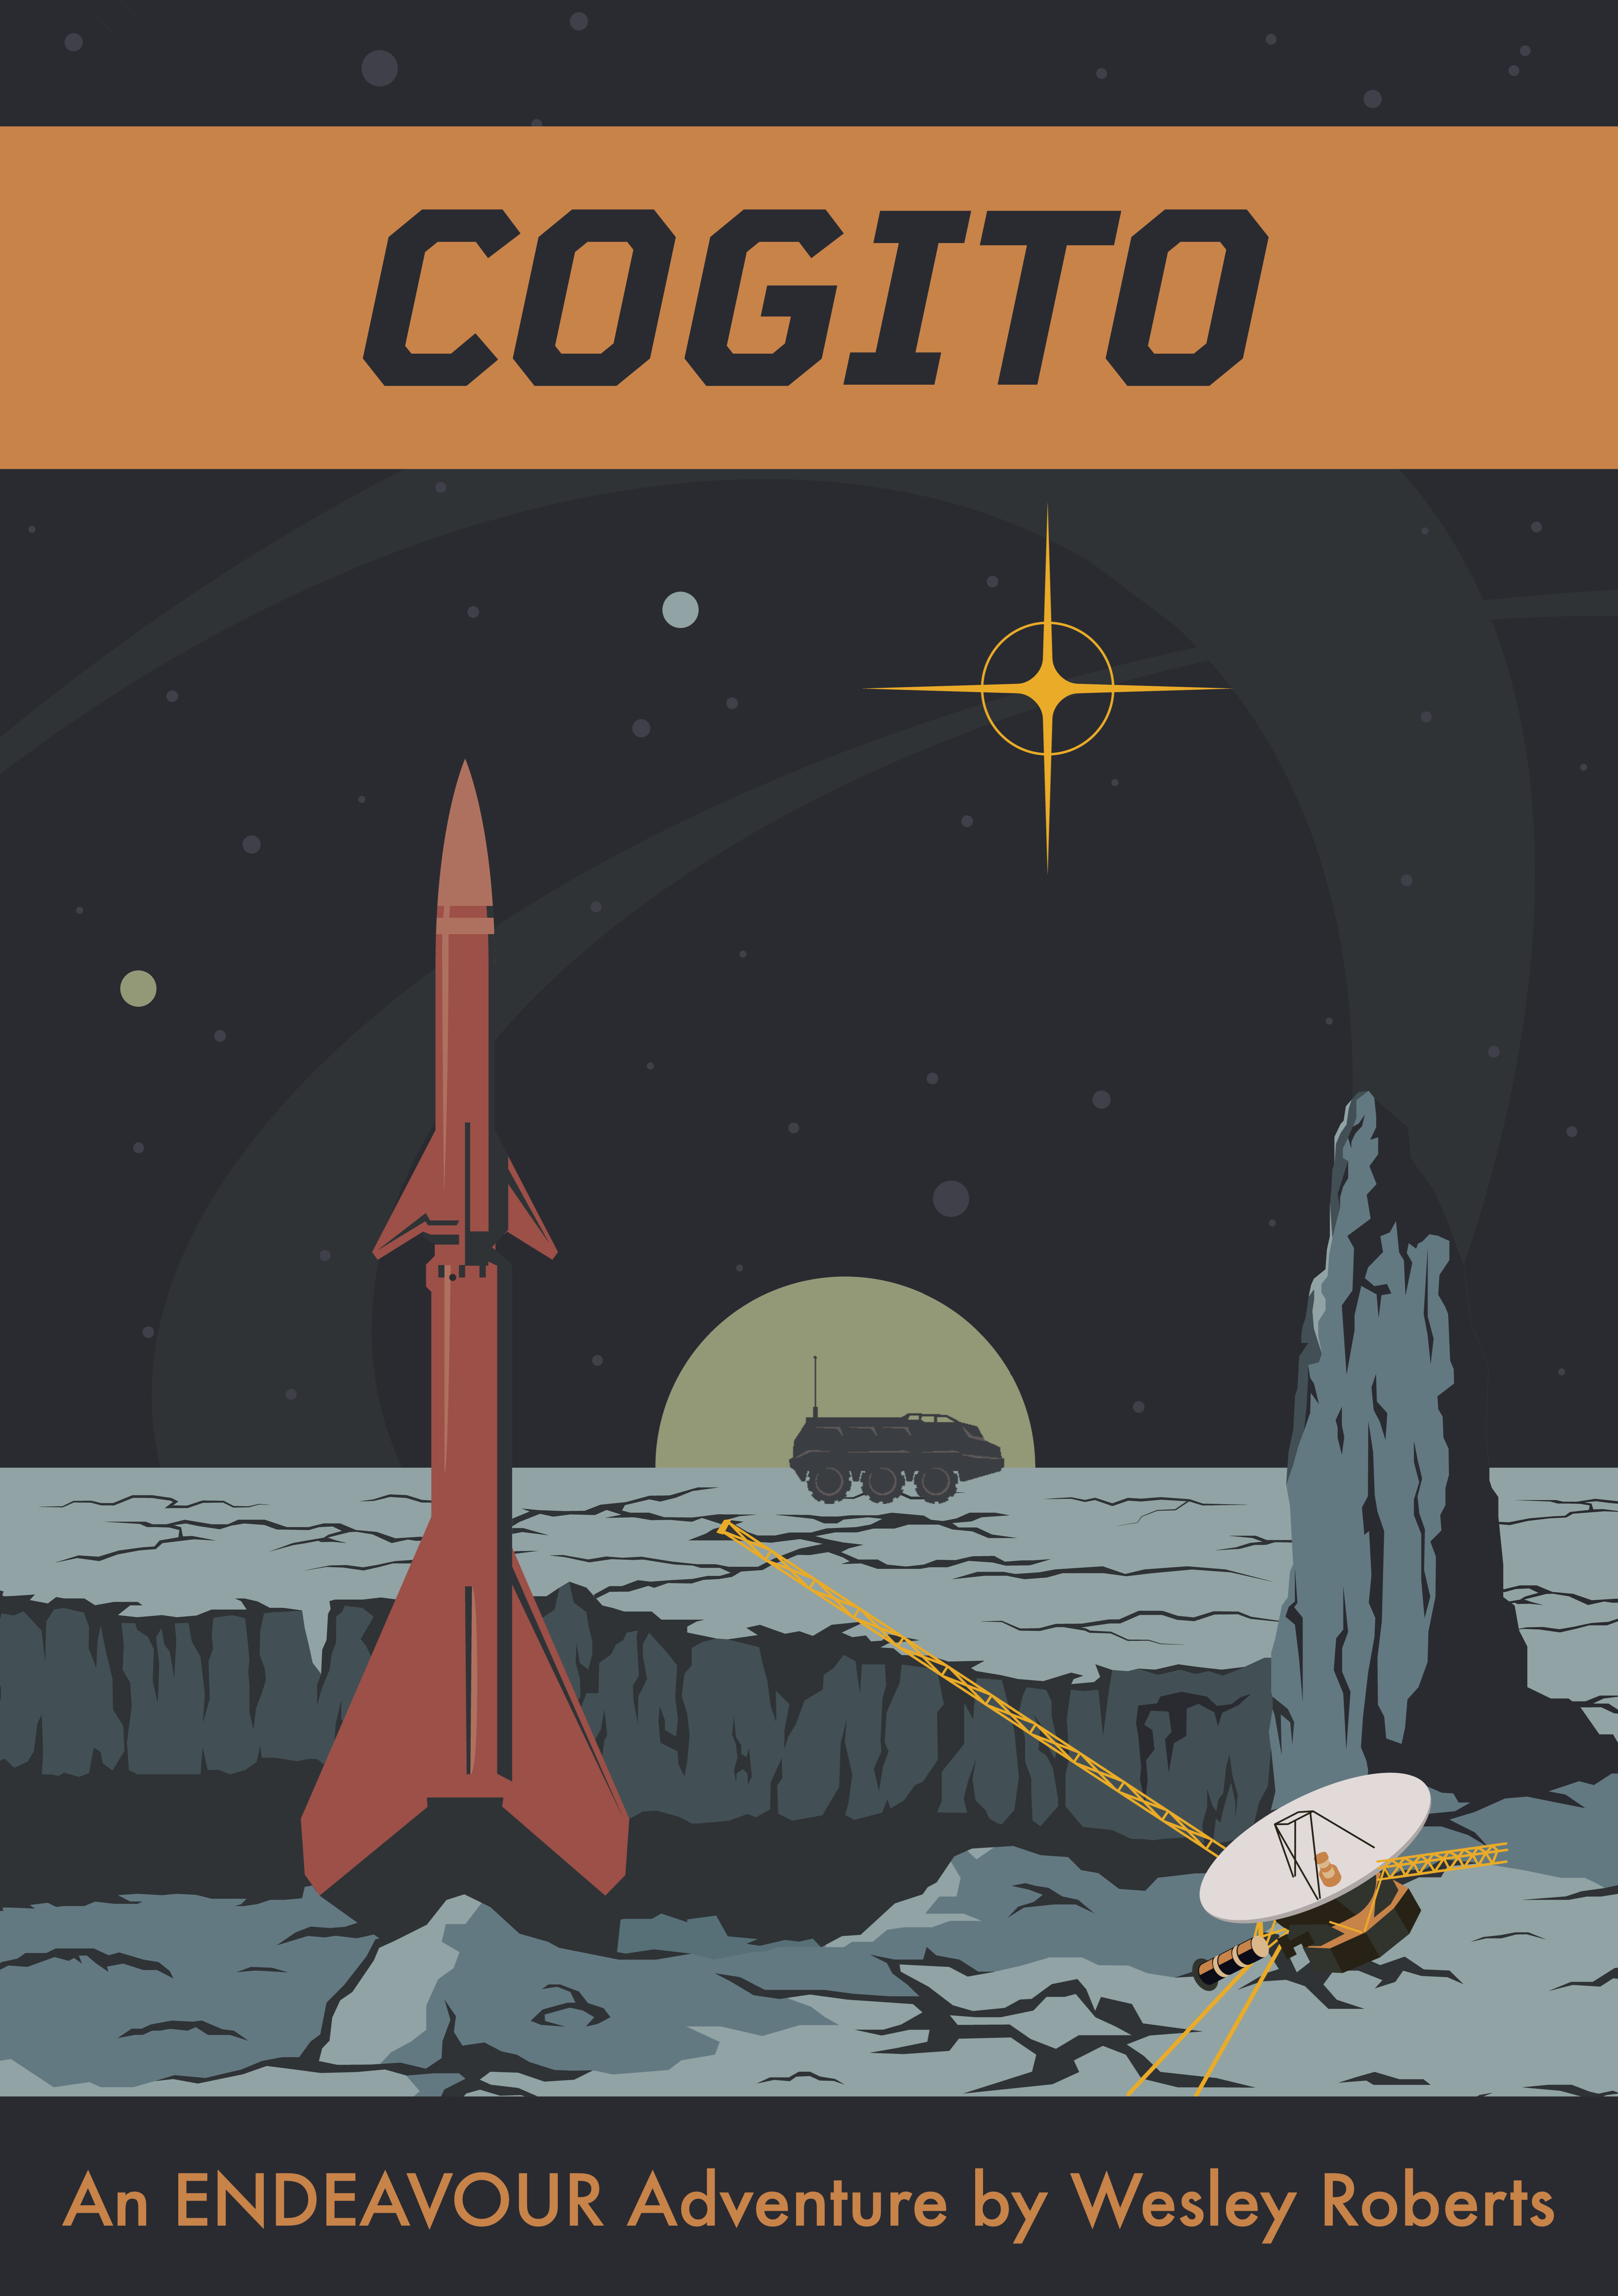
\includegraphics[width=\pagewidth, height=\pageheight]{Images/cogito_cover.png}};
\end{tikzpicture}
}
{
\colorlet{headfootcolor}{LCARS_ORANGE}
\phantom{a}

\newpage
}

\ClearShipoutPicture
\AddToShipoutPictureBG{
	\begin{tikzpicture}[remember picture, overlay]
	\pic () at (current page.center) {starfield};
		\node[endeavour_box, minimum width=12.6cm, minimum height=18.8 cm] at (current page.center) {};
	\end{tikzpicture}
}

\setcounter{page}{1}
\setmainfont{TeX Gyre Schola}
\normalsize
\raggedright

\section*{Cogito}
\textit{\textbf{Captain's Log:} Paradoxically, the oldest vessels that a spacefaring civilization sends into the void tend to be those that remain closest to their planets of origin. Indeed, despite having begun its journey nearly four hundred years ago, Voyager 1 \textemdash{} humanity's first interstellar probe \textemdash{} has only reached as far as the icy Oort cloud that orbits Sol.}

\textit{Astronomers have recently identified debris that threatens the ancient probe. As such, we have been assigned the task of recovering Voyager 1 so that it might be preserved in perpetuity. Accompanying us on our mission is Excellency Tamimi \textemdash{} the Terran Coordinator for Culture \textemdash{} who will be documenting our recovery efforts.}

\subsection*{Arrival}
At first glance, your viewport shows that you have arrived in a dense starfield, but soon you sense the chaotic dance of these innumerable jewels against the blackness of space.

The proximity alarm sounds, warning you of a spacecraft nearby. It's a centuries-old Terran ark, equipped with neither weapons nor a faster-than-light drive. 

\textbf{Ois\'in, captain of the Cogito} contacts you using an archaic communications device. He claims salvage rights to the Voyager 1, which has crashed into a nearby asteroid.

\subsubsection*{Close Encounter}
\begin{itemize}
	\item \textit{Will you try to convince Ois\'in to work together and cooperate with you to investigate the crash site?} \textbf{Leadership \& Negotiation} vs. \textbf{Ois\'in}.
	\item \textit{Or will you try to establish a stronger claim by sending a team to the crash site before Ois\'in can do the same?} \textbf{Strategy \& Tactics} vs. \textbf{Ois\'in}. 
\end{itemize}

\newpage

\subsection*{Trials}
\subsubsection*{Journalistic Ethics}
Excellency Tamimi sees the presence of the Cogito as an opportunity to add a layer of depth to the story they are telling about the recovery of Voyager 1. \textit{Can you convince them to find a nonexploitative way to tell their story?} \\ \textbf{Leadership \& Negotiation} vs. \textbf{Tamimi}.

\subsubsection*{The Dig}
Voyager 1 lies partially entombed under a large pile of rubble. It cannot be lifted remotely. \textit{Can you excavate the crash site so that Voyager 1 can be safely recovered?} \textbf{Operations \& Engineering} vs. \textbf{The Crash Site (2d10)}. During the operation, Ois\'in suffers a broken leg when he loses control of the rover that he is operating.

%\subsubsection*{Reluctant Patient}
%Ois\'in is reluctant to allow the Endeavour's medical staff to treat his injury. He stipulates that no pharmaceuticals be administered and that no broad-spectrum scans be performed. \textit{Can you discover why Ois\'in is so reluctant to let you help him?} \textbf{Science \& Medicine} vs. \textbf{Ois\'in}.

\subsubsection*{Persona Non Grata}
While treating Ois\'in's injury, you discover that his genome is modified in ways that would preclude him from being granted citizenship anywhere within the Interstellar Confederation. \textit{Can you discover a way to neutralize Ois\'in's dangerous genetic modifications?} \textbf{Science \& Medicine} vs. \textbf{Ois\'in}.

\subsection*{Crisis}
Ois\'in asks that the crew of the Cogito be placed back into stasis and allowed to continue their journey alongside Voyager 1. Tamimi asks instead that that Voyager 1 be returned to Earth and the crew of the Cogito be ``rescued''. 

\begin{itemize}
	\item \textit{Will you side with Ois\'in?} \textbf{Threats:} Ois\'in suffers an adverse reaction to being put back in stasis. Tamimi's broadcast contains evidence of Ois\'in's abnormal genetics.
	\item \textit{Or will you side with Tamimi?} \textbf{Threats:} Ois\'in destroys Voyager 1 in protest. The fate of the Cogito becomes the focal point of a populist movement on Earth.% to
%withdraw from the Interstellar Confederation.
%and legalize genetic manipulation.
\end{itemize}

\newpage

\subsection*{Characters}
\begin{description}
	\item[Tamimi (d12):] Terran Coordinator for Culture (d10), \\ Powerful (d10), Persuasive (d10), Loyal (d8).
	\item[Ois\'in (d10):] Captain of the Cogito (d10), \\ Determined (d10), Indefatigable (d10), Cunning (d8).
\end{description}

\subsection*{Places}
\begin{description}
	\item[The Oort Cloud:] A sparse cloud of rocks and ice that orbit far from Sol in a spherical shell around the system.
	\item[The Cogito:] An antiquated ark. Designed to support twenty-seven people, the Cogito is approximately two hundred years old and bears numerous battle scars. On board are Ois\'in's wife, Niamh, and their three children.
	\item[The Crash Site:] A crater on a large asteroid in which Voyager 1 lies partially entombed by a large pile of rubble.
\end{description}

\subsection*{Mysteries}
\begin{description}
	\item[The crew of the Cogito are political refugees.] \phantom{a} \\ They fled from Earth to escape persecution that they suffered because of their genetic modifications.
Ois\'in is curious whether the modern Terran Civilization is more open-minded than it was in his time. \textit{How have the crew of the Cogito been modified?  Why were those changes made?}
	\item[The Cogito followed Voyager 1 to this place.] \phantom{a} \\ Ois\'in believed anyone who could recover Voyager 1 would welcome his crew into their civilization. The Interstellar Confederation, however, has outlawed the kinds of modifications that affect the crew of the Cogito. They will be unwelcome in any of its member civilizations.
\textit{Why are prohibitions of these genetic modifications so ubiquitous?}
%\textit{Why won't the Interstellar Confederation welcome the crew of the Cogito into modern society?}
\end{description}

\newpage

\section*{Acknowlegements}
Much of the look and feel of \ENDEAVOUR{} is derived from its art, all of which was created by \textbf{svekloid}. This art was assembled from multiple collections available online at \href{http://shutterstock.com}{shutterstock.com} and then modified by Michael Purcell.  

\subsection*{Playtesters} \label{subsection:playtesters}
The following people helped to create \ENDEAVOUR{} by playing early versions of the game and providing invaluable feedback.\vspace{-1.75ex}
\begin{multicols}{2}
\begin{itemize}[noitemsep]
  \item Keydan Bruce
  \item Dannielle Harden
  \item Andrew Hellyer
%  \item Sarah Hewat
%  \item Scott Joblin
%  \item Sen-Foong Lim
  \item David McKenzie
%  \item Holly Moore
  \item Paul Murray
%  \item David Purcell
%  \item Heidi Purcell
  \item Kira Purcell
  \item Luke Purcell
  \item Meagan Purcell
%  \item Steve Purcell
%  \item Jason Stark
  \item Jo Stephenson
%  \item Pieter Vismans
  \item Brett Witty
  \item Bevis Worcester
  \item Evan Worcester
\end{itemize}
\end{multicols}

\subsection*{Design Tools} \label{subsection:design-tools}
The following tools were used to create this document:
\begin{description}[font=\normalfont\textbullet\space, noitemsep, topsep=-1ex]
	\item[LuaLaTeX:] Typesetting and layout.
	\item[TikZ:] Diagrams and art.
\end{description}
\vspace{1ex}
The fonts used are {\setmainfont{TT Mussels-BoldItalic} TT~Mussels~Bold~Italic},  \textsf{Futura}, and TeX~Gyre~Schola (cf. Century Schoolbook).

\vfill

\begin{tabular}{@{}m{7.775cm}@{\hspace*{0.375cm}}>{\centering\arraybackslash}m{2.6cm}@{}}
\textbf{Contact:} \href{mailto:endeavour.ttrpg@gmail.com}{endeavour.ttrpg@gmail.com}\newline \phantom{This is a test, only a test.} \newline \footnotesize{For use with the \textsc{Paragon} system, ©2020\newline \textbf{John Harper \& Sean Nittner}. \href{http://agon-rpg.com}{AGON-RPG.com}} & \includegraphics[scale=0.175]{Images/paragon_logo_mark.png} \\[5ex]
\footnotesize{This work is licensed under a Creative Commons \newline ``Attribution-ShareAlike 4.0 International'' license.} & \Huge{\doclicenseIcon}
\end{tabular}

\newpage

\thispagestyle{empty}

\tikzset{starfield/.pic={
	\node () at (current page.center) {
\includegraphics[width=\pagewidth, height=\pageheight]{Images/starfield.png}};
}}

\ClearShipoutPicture
\AddToShipoutPictureBG{
	\begin{tikzpicture}[remember picture, overlay]
	\pic () at (current page.center) {starfield};
	\end{tikzpicture}
}

\phantom{a}

\end{document}